% \title{Apunte de Matemáticas Discretas CC3101:\\ 
% Relaciones de Recurrencia  Clase 13}
% % \title{Ejercicios Lógica e Inducción}
% \author{Andrés Abeliuk}
% \date{}
% \maketitle


\section{Relaciones de Recurrencia }

\subsection{Introducción}

Las \textbf{relaciones de recurrencia} son una herramienta poderosa en matemáticas discretas para definir y analizar secuencias de manera recursiva. Estas relaciones aparecen frecuentemente en análisis de algoritmos, conteo, estructuras de datos y resolución de problemas combinatorios.

\begin{definitionblock}{Definición: Relación de recurrencia}
Una relación de recurrencia para una secuencia $\langle a_n
\rangle_{n \geq 0}$ es una ecuación que expresa $a_n$ en términos de
sus predecesores $a_{n-1}, a_{n-2}, \ldots, a_0$.

\medskip

Para determinar unívocamente la secuencia debemos dar explícitamente
los valores de un número finito de los primeros términos de la
secuencia. Éstos se conocen como las \textbf{condiciones iniciales} de
la recurrencia.
\end{definitionblock}

En otras palabras, una relación de recurrencia no es nada más que una \textbf{definición recursiva} de una secuencia $\langle a_n \rangle_{n \geq 0}$.


\begin{exampleblock}{Ejemplo: crecimiento de un sueldo}
Laura recibe un sueldo inicial de $2000$ y un aumento del $10\%$ mensual. Sea $a_n$ el sueldo en el mes $n$:
\begin{align*}
a_1 &= 2000 \\
a_n &= 1.1 \cdot a_{n-1} \quad \forall n \geq 2
\end{align*}
\noindent La forma cerrada es: $a_n = 2000 \cdot 1.1^{n-1}$
\end{exampleblock}

\begin{exampleblock}{Ejemplo: Fibonacci}
La sucesión de Fibonacci es un ejemplo clásico:
\[
f_0 = 0, \quad f_1 = 1, \quad f_n = f_{n-1} + f_{n-2}, \text{ para } n \geq 2.
\]
\end{exampleblock}


\subsection*{Aplicaciones en problemas de conteo}

\begin{exampleblock}{Problema: Subiendo la escalera}
\noindent
\begin{minipage}[c]{0.74\textwidth}
\vspace*{0pt}
\centering
Se desea subir una escalera de $n$ escalones. En cada paso se puede subir uno o dos escalones. ¿De cuántas maneras distintas puede se llegar al escalón $n$?
\end{minipage}%
\hfill
\begin{minipage}[c]{0.24\textwidth}
\centering
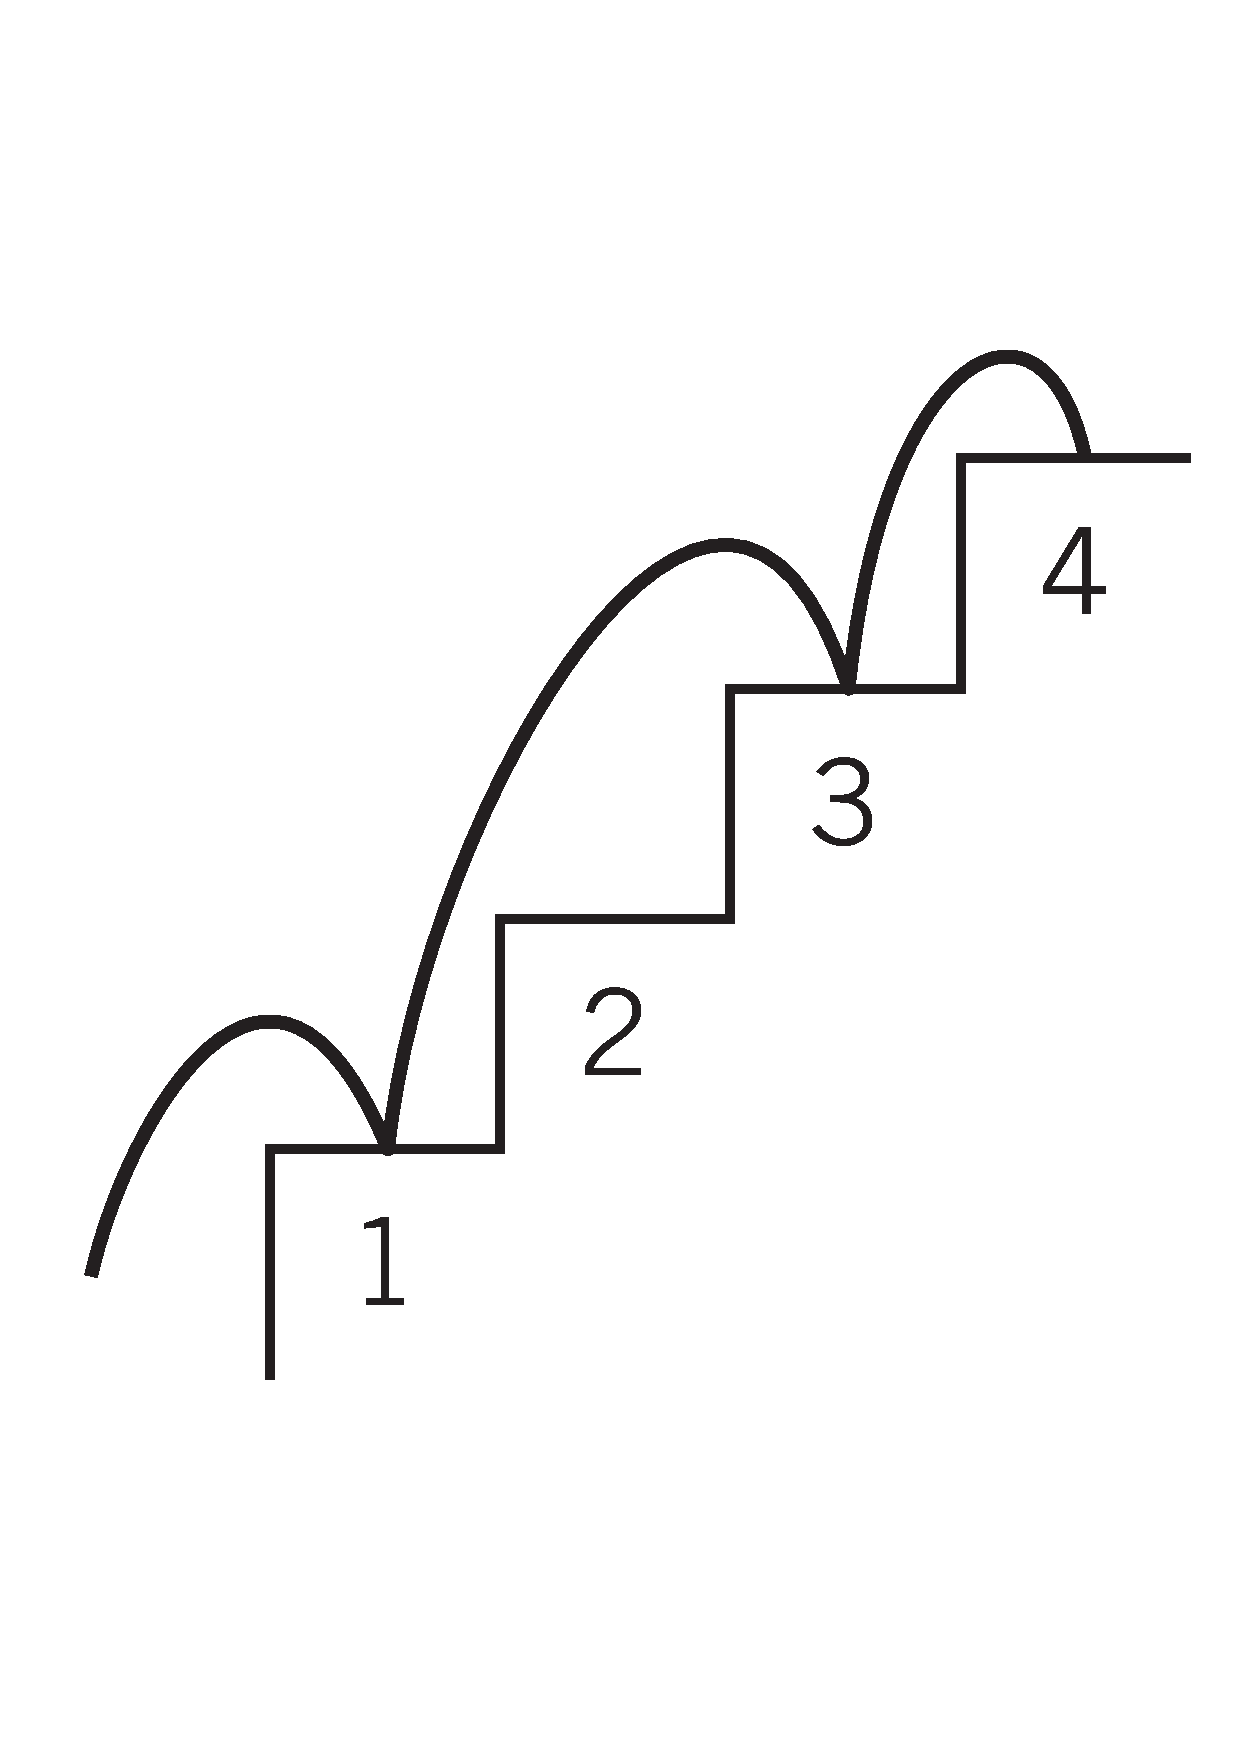
\includegraphics[width=0.8\linewidth]{Figures/stairs.pdf}
\end{minipage}
\end{exampleblock}
\noindent \textbf{Solución:}\\
Para $n = 1$ hay una única forma: dar un paso de un escalón.\\
Para $n = 2$ hay dos formas:
\begin{itemize}
\item dar dos pasos de un escalón,
\item dar un solo paso de dos escalones.
\end{itemize}
Para ver de cuántas maneras se puede subir una escalera de $n\geq 3$ escalones hacemos un análisis de casos:
\begin{itemize}
\item Si el primer paso es de un escalón, restan $n-1$: hay $a_{n-1}$ formas de completarlo.
\item Si el primer paso es de dos escalones, restan $n-2$: hay $a_{n-2}$ formas.
\end{itemize}
Por la regla de la suma:
\begin{equation}
a_n = a_{n-1} + a_{n-2} \quad \text{para } n \geq 3
\end{equation}
Resumiendo, tenemos la siguiente relación de recurrencia para calcular el número de formas $a_n$ en las que Juan puede subir una escalera de $n$ escalones:
\begin{align*}
  a_1 &~=~ 1\\
  a_2 &~=~ 2\\
  a_n &~=~ a_{n-1} + a_{n-2} \quad \forall n\geq 3
\end{align*}
Esta es la \textbf{sucesión de Fibonacci}, y tiene
muchas aplicaciones en problemas de conteo.



\begin{exampleblock}{Ejercicios: Palabras binarias sin 00 consecutivos}
Sea $a_n$ el número de palabras binarias de largo $n$ sin dos 
\end{exampleblock}
\noindent \textbf{Solución:}\\
Para construir una palabra binaria válida de largo $n$ (es decir, sin ocurrencias de $00$), consideramos los posibles caracteres finales:
\begin{itemize}
  \item Si la palabra termina en \texttt{1}, entonces el prefijo de largo $n - 1$ puede ser cualquier palabra válida. Hay $a_{n-1}$ de estas.
  \item Si termina en \texttt{0}, entonces el penúltimo carácter debe ser \texttt{1} (para evitar $00$). Por lo tanto, el prefijo de largo $n - 2$ puede ser cualquier palabra válida, seguida de \texttt{10}. Hay $a_{n-2}$ de estas.
\end{itemize}
Por la regla de la suma:
\[ a_n = a_{n-1} + a_{n-2} \quad \forall n\geq 3 \]
Condiciones iniciales:
\begin{align*}
a_1 &~=~ 2 \quad (\texttt{0}, \texttt{1}) \\
a_2 &~=~ 3 \quad (\texttt{01}, \texttt{10}, \texttt{11})
\end{align*}
Esta es nuevamente la \textbf{sucesión de Fibonacci}, pero con condiciones iniciales distintas.



\begin{exampleblock}{Ejercicio: Conexiones entre personas}
Cada vez que una nueva persona entra a una reunión, saluda a todas las personas que ya están. ¿Cuántos apretones de manos se han dado después de que han llegado $n$ personas (una por una)?
\end{exampleblock}
\noindent \textbf{Solución:}\\
Sea $a_n$ el número total de apretones de manos después de que han llegado $n$ personas. Cada nueva persona saluda a todas las que ya llegaron, es decir, realiza $n-1$ apretones. Entonces:
\begin{align*}
a_1 &= 0 \\
a_n &= a_{n-1} + (n - 1) \quad \text{para } n \geq 2
\end{align*}
% \noindent Esta secuencia representa los números triangulares desplazados.


% Ejercicio propuesto: Regiones en el plano
% Dibujando $n$ rectas con intersecciones generales, sea $a_n$ el número de regiones:
% % \begin{align*}
% % a_1 &= 2 \
% % a_n &= a_{n-1} + n \quad (n \geq 2)
% % \end{align*}




\begin{exampleblock}{Problema: Torres de Hanoi}
\noindent
\begin{minipage}[c]{0.74\textwidth}
\vspace*{0pt}
\centering
Las Torres de Hanoi son un puzzle que
consiste de 3 barras montadas en un tablero y una serie de discos de diferente tamaño.  
Inicialmente los discos estás dispuestos como se muestran a continuación:
El objetivo del puzzle es pasar todos los discos a otra de las barras con las siguientes restricciones:
\begin{itemize}
\item Los discos deben quedar dispuestos de la misma manera (en orden)
  %
\item Los discos se pueden pasar entre las barras, de a uno (por lo
  que en cada paso se puede mover sólo el disco superior de cada barra) 
  %
\item Al depositar un disco en otra barra, no puede quedar sobre otro de menor tamaño.
\end{itemize}
 ¿Cuál es la menor cantidad de movimientos $h_n$ que debo hacer para resolver el puzzle desde una configuración inicial con $n$ discos?
\end{minipage}%
\hfill
\begin{minipage}[c]{0.24\textwidth}
\centering
 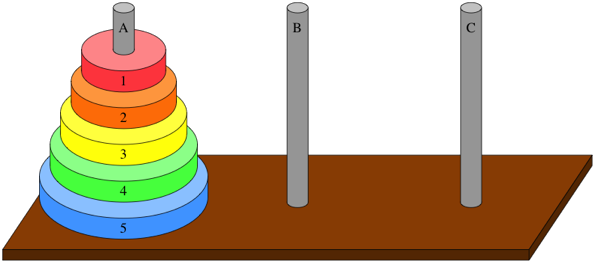
\includegraphics[width=\textwidth]{Figures/HanoiStarting.png}\hspace{1cm}
\end{minipage}
\end{exampleblock}
\noindent \textbf{Solución:}\\
La clave está en observar la estructura recursiva del problema.

\begin{itemize}
\item Para mover una torre de $n$ discos desde la barra origen a la barra destino:
\begin{enumerate}
\item Primero movemos los $n-1$ discos superiores a la barra auxiliar (requiere $h_{n-1}$ movimientos).
\item Luego movemos el disco más grande directamente a la barra destino (1 movimiento).
\item Finalmente, movemos los $n-1$ discos desde la barra auxiliar a la barra destino (otros $h_{n-1}$ movimientos).
\end{enumerate}
\end{itemize}

Esto da lugar a la siguiente relación de recurrencia:
\begin{align*}
  h_n &~=~ 2h_{n-1} + 1 \quad \forall n\geq 2 \\
  h_1 &~=~1 
\end{align*}
\medskip

Puede verificarse fácilmente que $$ h_n~=~2^n-1 $$ es la forma cerrada(o solución) de la recurrencia. 

\begin{exampleblock}{Asociación de productos (Números de Catalán)}
Sea $c_n$ el número de formas de parentizar $n$ factores $a_1 \cdot a_2 \cdot \cdots \cdot a_{n-1} \cdot a_n$. Demostrar la siguiente recurrencia:
\begin{align*}
c_1 &= 1 \\
c_n &= \sum_{i=1}^{n-1} c_i \cdot c_{n-i} \quad (n \geq 2)
\end{align*}
\end{exampleblock}
\noindent \textbf{Solución:}\\
Si se agrupa el producto como $(A) \cdot (B)$, donde:
\begin{itemize}
\item $A$ es un subproducto de los primeros $k$ factores,
\item $B$ es el subproducto de los $n-k$ restantes,
\end{itemize}
\noindent entonces hay $c_k$ formas de parentizar $A$ y $c_{n-k}$ formas de parentizar $B$, lo que da $c_k \cdot c_{n-k}$ formas para esa partición. Sumando sobre todas las posibles particiones (de $k = 1$ a $n-1$) obtenemos la recurrencia.

Esta sucesión es conocida como los \textbf{números de Catalán}, denotados habitualmente por $C_{n-1}$.
\textbf{Fórmula cerrada:}
\[
c_n = \frac{1}{n} \binom{2n - 2}{n - 1} = \frac{(2n - 2)!}{n!(n - 1)!}
\]

\subsection{Sistemas de relaciones de recurrencia}
En muchos problemas de conteo, la cantidad total de soluciones no depende solamente de un valor anterior en la secuencia, sino que involucra el resultado de varias secuencias interrelacionadas. En estos casos, hablamos de 	\textbf{sistemas de relaciones de recurrencia}. A diferencia de las relaciones simples, estos sistemas describen conjuntos de secuencias que se definen mutuamente.

\begin{exampleblock}{Ejercicio: Piezas de dominó y cuadrículas}
\textbf{Enunciado:} ¿De cuántas maneras, $F_n$, se puede llenar una cuadrícula de $3 \times n$ con piezas de dominó de $2 \times 1$?
\end{exampleblock}
\noindent \textbf{Solución:}\\
Para determinar $F_n$ analizamos cómo puede completarse la \textit{última columna} de la cuadrícula. Hay tres configuraciones típicas (ver Figura~\ref{fig:cuadricula_1}):
\begin{figure}[h]
\centering
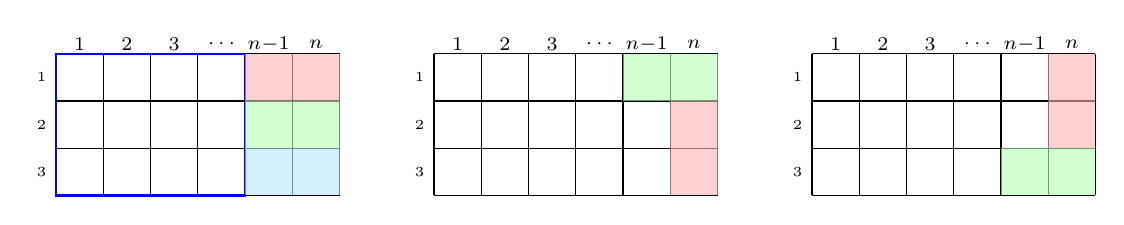
\begin{tikzpicture}[scale=0.6]

% === Diagrama 1 ===
\begin{scope}[shift={(0,0)}]
  % grid
  \foreach \x in {0,...,6} {
    \draw (\x, 0) -- (\x, 3);
  }
  \foreach \y in {0,...,3} {
    \draw (4,\y) -- (6,\y); % final columns
  }
  \foreach \y in {0,...,3} {
    \draw (0,\y) -- (6,\y);
  }
  % Labels
  \node at (0.5,3.2) {\scriptsize 1};
  \node at (1.5,3.2) {\scriptsize 2};
  \node at (2.5,3.2) {\scriptsize 3};
  \node at (3.5,3.2) {\scriptsize $\cdots$};
  \node at (4.5,3.2) {\scriptsize $n{-}1$};
  \node at (5.5,3.2) {\scriptsize $n$};

  \node[anchor=east] at (0,2.5) {\tiny 1};
  \node[anchor=east] at (0,1.5) {\tiny 2};
  \node[anchor=east] at (0,0.5) {\tiny 3};

  % Highlight rectangles
  \draw[thick,blue] (0,0) rectangle (4,3);
  \fill[red!30,opacity=0.6] (4,2) rectangle (6,3);
  \fill[green!30,opacity=0.6] (4,1) rectangle (6,2);
  \fill[cyan!30,opacity=0.6] (4,0) rectangle (6,1);
\end{scope}

% === Diagrama 2 ===
\begin{scope}[shift={(8,0)}]
  % grid
  \foreach \x in {0,...,6} {
    \draw (\x, 0) -- (\x, 3);
  }
  \foreach \y in {0,...,3} {
    \draw (4,\y) -- (6,\y);
  }
  \foreach \y in {0,...,3} {
    \draw (0,\y) -- (6,\y);
  }

  % Labels
  \node at (0.5,3.2) {\scriptsize 1};
  \node at (1.5,3.2) {\scriptsize 2};
  \node at (2.5,3.2) {\scriptsize 3};
  \node at (3.5,3.2) {\scriptsize $\cdots$};
  \node at (4.5,3.2) {\scriptsize $n{-}1$};
  \node at (5.5,3.2) {\scriptsize $n$};

  \node[anchor=east] at (0,2.5) {\tiny 1};
  \node[anchor=east] at (0,1.5) {\tiny 2};
  \node[anchor=east] at (0,0.5) {\tiny 3};

  % Highlight rectangles
  
  \fill[red!30,opacity=0.6] (5,0) rectangle (6,2);
  \fill[green!30,opacity=0.6] (5,2) rectangle (6,3);
   \fill[green!30,opacity=0.6] (4,2) rectangle (5,3);
\end{scope}

% === Diagrama 3 ===
\begin{scope}[shift={(16,0)}]
  % grid
  \foreach \x in {0,...,6} {
    \draw (\x, 0) -- (\x, 3);
  }
  \foreach \y in {0,...,3} {
    \draw (4,\y) -- (6,\y);
  }
  \foreach \y in {0,...,3} {
    \draw (0,\y) -- (6,\y);
  }

  % Labels
  \node at (0.5,3.2) {\scriptsize 1};
  \node at (1.5,3.2) {\scriptsize 2};
  \node at (2.5,3.2) {\scriptsize 3};
  \node at (3.5,3.2) {\scriptsize $\cdots$};
  \node at (4.5,3.2) {\scriptsize $n{-}1$};
  \node at (5.5,3.2) {\scriptsize $n$};

  \node[anchor=east] at (0,2.5) {\tiny 1};
  \node[anchor=east] at (0,1.5) {\tiny 2};
  \node[anchor=east] at (0,0.5) {\tiny 3};

  % Highlight rectangles
  % \draw[thick,blue] (0,0) rectangle (5,3);
  \fill[red!30,opacity=0.6] (5,2) rectangle (6,3);
  \fill[red!30,opacity=0.6] (5,1) rectangle (6,2);
  \fill[green!30,opacity=0.6] (4,0) rectangle (6,1);
\end{scope}

\end{tikzpicture}
\caption{Tres formas posibles de completar la última columna de una cuadrícula $3 \times n$ usando piezas de dominó.}
\label{fig:cuadricula_1}
\end{figure}

Notar que la cantidad de maneras de llenar la cuadrícula en los últimos dos casos es la misma, ya que son simétricas. Llamemos $G_{n-1}$ a ese
número.  Luego, por la regla de la suma tenemos que
\[
F_n ~=~F_{n-2} + 2 G_{n-1}
\]

Nuevamente, hacemos análisis de casos sobre cómo puede rellenarse la columna más
pequeña de $G_{n}$. Vemos que hay dos maneras (ver Figura~\ref{fig:cuadricula_1}). En el primer caso, la forma de cubrir la subestructura es equivalente a $F_{n-1}$ y en el segundo caso, a $G_{n-2}$. Por lo tanto:
y por la regla de la suma resulta que
\[
  G_n ~=~ F_{n-1} + G_{n-2}
  \]
\begin{figure}[h]
\begin{center}
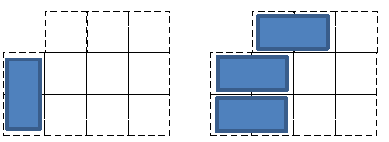
\includegraphics[width=0.4\textwidth]{Figures/tilingpattercases.png}  
\caption{Dos formas posibles de completar la última columna de una cuadrícula $G_{n}$ usando piezas de dominó.}
\label{fig:cuadricula_1}
\end{center}
\end{figure}
 Agregando las condiciones iniciales tenemos que
  \begin{align*}
    F_n &~=~F_{n-2} + 2 G_{n-1} \quad \forall n \geq 2\\
    F_0&~=~1\qquad F_1~=~0\\  
    G_n &~=~ F_{n-1} + G_{n-2}  \quad \forall n \geq 2\\
    G_0&~=~0\qquad G_1~=~1\\  
  \end{align*}
  lo que nos da un sistema de recurrencias para definir $F_n$. 


\subsection{Ejercicios propuestos}

\begin{itemize}
\item \textbf{Ejercicio:} Un string de números decimales es válido si contiene un número par de ceros. Use una relación de recurrencia para definir $c_n$, el número de strings válidos de largo $n$.
\medskip
\item \textbf{Ejercicio:} Defina recursivamente la sucesión ${a_n}$ que da la cantidad de strings de largo $n$ que no tienen dos ceros consecutivos.
\item \textbf{Ejercicio:} Supongamos que dibujamos $n$ rectas en una hoja de papel de manera que todo par de líneas se intersectan (pero no hay tres líneas que se intersectan en un único punto). ¿En cuántas regiones queda dividido el plano?
\end{itemize}